\section{Evaluation}
We deployed \xxx Mac OS X x86 platform, with the Model code MacBookPro9,2.
The model has the Intel Core i5-3210M CPU with 2 cores and 4 thread,
10GB DDR3 memory, and we replace the hard disk with a 1T ssd.

We first presents the performance impact of the live deployment of Argus.
We demonstrate the overhead of our tracing tool intruduced, regarding the storage, memory and CPU usage.
Then we list the softwares which trigger spinning wait cursors in MacOs and the root cause we figure out with our framework.
At the end, we summaries the tedious work that our tool can take over from the user and make the diagnosis much easier in the wild.

\begin{figure}[tb]
    \centering
    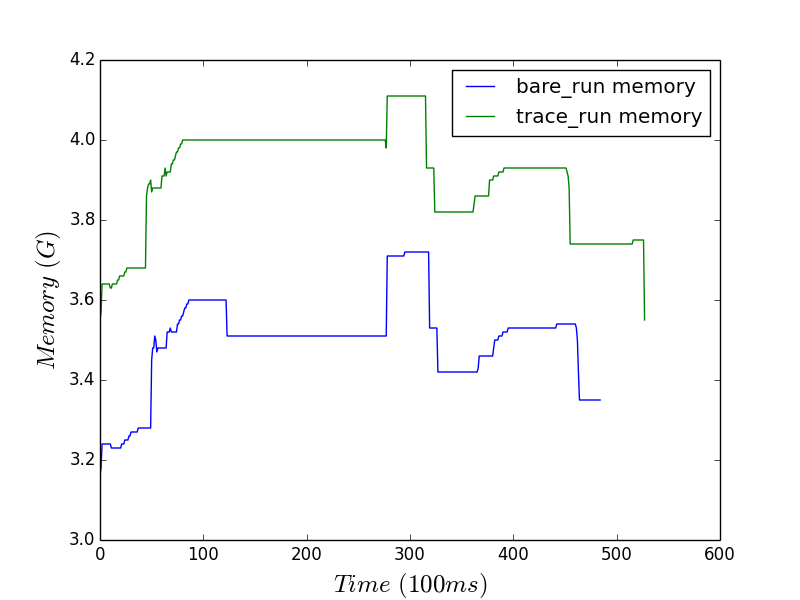
\includegraphics[width=1.0\linewidth]{ibench_memory_compare.png}
    \caption{Memory overhead with tracing.}
    \label{fig:ibench_memory_overhead}
\end{figure}

\begin{figure}[tb]
    \centering
    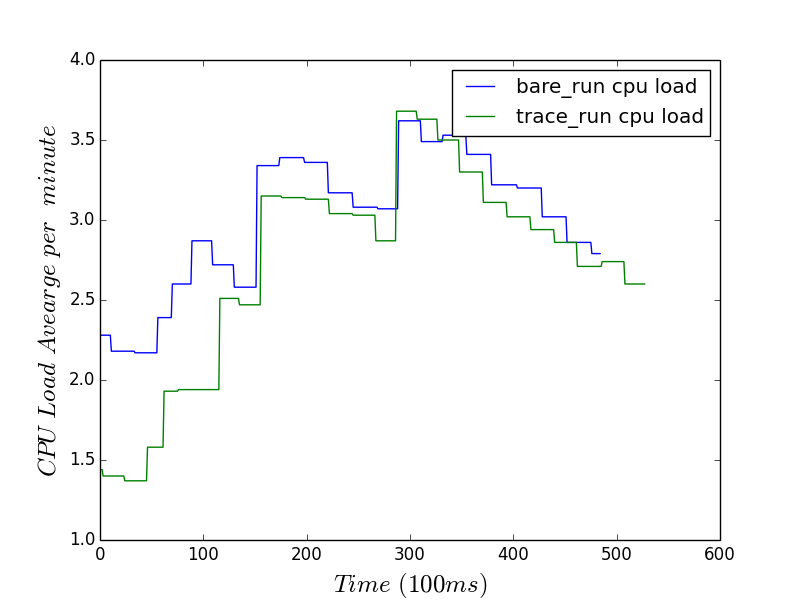
\includegraphics[width=1.0\linewidth]{ibench_cpuload_compare.png}
    \caption{CPU overhead with tracing.}
    \label{fig:ibench_cpu_overhead}
\end{figure}

\subsection{iBench}
iBench is a synthetic micro benchmark for the CPU and memory performance on MacOS.
We run the suite in the machine with and without \xxx enabled respectively,
and collect the memory usage and cpu load for every 100 millisecons.
Figure \ref{fig:ibench_memory_overhead} shows in \xxx, about 512M more memory in the footprint on \xxx,
which is consistent with the default size of the internal buffer used to collect events in Apple's tracing facility.
We also notice that the time cost of the two runs nearly the same.
Figure \ref{fig:ibench_cpu_overhead} illustrate the cpu load every minutes for both settings.
It supports the same conclusion that
users can hardly realize the performance impact of our system.

\subsection{Real-world Applications}
With \xxx deployed in the paltform, the tracing tool is running in the background 24X7.
Once the spinning cursor appeers on the screen,
we store the tracing data for the root cause analysis.
 
The list of real-world softwares includes TextEdit, CodEdit, Notes, Hopper Disassembler, Installer, Squel Pro, GetiPlayerAutomator.
\begin{table}[h]
\begin{tabular}{|l|c|c|}
Application & Reproduce Method & Root Cause\\
\hline
TextEdit & & \\
CoEdit & & \\
Notes & & \\
HopperDiassembler & & \\
Installer & &\\
Squel Pro & & \\
%GetiPlayerAutomator & &\\
\end{tabular}
\caption{Diagnosis of Daily Softwares}
\label{tab:disagnosis of daily softwares}
\end{table}


%\begin{itemize}
%\item tracing overhead
	%\begin{itemize}
	%\item memory and CPU usage on top, while running ibench with and without our tracing enabled
	%\item memory and CPU usage on top, while running the listed real world applications with and without our tracing enabled
	%\item how much times it takes to filled the buffer we fixed 2G
	%\item how many events recorded in the buffer
	%\end{itemize}
%\item number of edges and nodes in the graphs and portions of data the user need to examine to figure out the root cause.
%\end{itemize}
